% \iffalse
\let\negmedspace\undefined
\let\negthickspace\undefined
\documentclass[journal,12pt,twocolumn]{IEEEtran}
\usepackage{float}
\usepackage{circuitikz}
\usepackage{cite}
\usepackage{amsmath,amssymb,amsfonts,amsthm}
\usepackage{algorithmic}
\usepackage{graphicx}
\usepackage{textcomp}
\usepackage{xcolor}
\usepackage{txfonts}
\usepackage{listings}
\usepackage{amsmath}
\usepackage{enumitem}
\usepackage{mathtools}
\usepackage{gensymb}
\usepackage{comment}
\usepackage[breaklinks=true]{hyperref}
\usepackage{tkz-euclide} 
\usepackage{listings}
\usepackage{gvv}                                        
\def\inputGnumericTable{}                                 
\usepackage[latin1]{inputenc}                                
\usepackage{color}                                            
\usepackage{array}                                            
\usepackage{longtable}                                       
\usepackage{calc}                                             
\usepackage{multirow}                                         
\usepackage{hhline}                                           
\usepackage{ifthen}                                           
\usepackage{lscape}
\newtheorem{theorem}{Theorem}[section]
\newtheorem{problem}{Problem}
\newtheorem{proposition}{Proposition}[section]
\newtheorem{lemma}{Lemma}[section]
\newtheorem{corollary}[theorem]{Corollary}
\newtheorem{example}{Example}[section]
\newtheorem{definition}[problem]{Definition}
\newcommand{\BEQA}{\begin{eqnarray}}
\newcommand{\EEQA}{\end{eqnarray}}
\newcommand{\define}{\stackrel{\triangle}{=}}
\theoremstyle{remark}
\newtheorem{rem}{Remark}
\begin{document}

\bibliographystyle{IEEEtran}
\vspace{3cm}
\title{Audio Filter}
\author{EE23BTECH11046 - Poluri Hemanth$^{*}$% <-this % stops a space
}
\maketitle
\newpage
\bigskip
\renewcommand{\thefigure}{\arabic{figure}}
\renewcommand{\thetable}{\theenumi}

\bibliographystyle{IEEEtran}
\begin{enumerate}

\section{SOFTWARE INSTALLATION}
\item Run the following commands
\begin{lstlisting}
sudo apt-get update
sudo apt-get install libffi-dev libsndfile1 python3-scipy  python3-numpy python3-matplotlib 
sudo pip install cffi pysoundfile 
\end{lstlisting}
\section{Digital Filter}
\label{original_audio}
\item The audio file with noise to be filtered can be downloaded from
\begin{lstlisting}
$https://github.com/hemanth23ee/ASSIGNMENTS/blob/main/Audio%20filter%20assignment/codes/Song.wav
\end{lstlisting}
\item 
\label{code_filtering}
A Python Code is written to achieve Audio Filtering 
\lstinputlisting{./codes/audio_filter.py}\label{audio_filter.46}

\item 
\label{Visualization}


The frequencies of audio with noise are observed with help of spectrogram from \href{https://academo.org/demos/spectrum-analyzer}{\url{https://academo.org/demos/spectrum-analyzer}}.\\

\begin{figure}[H]
    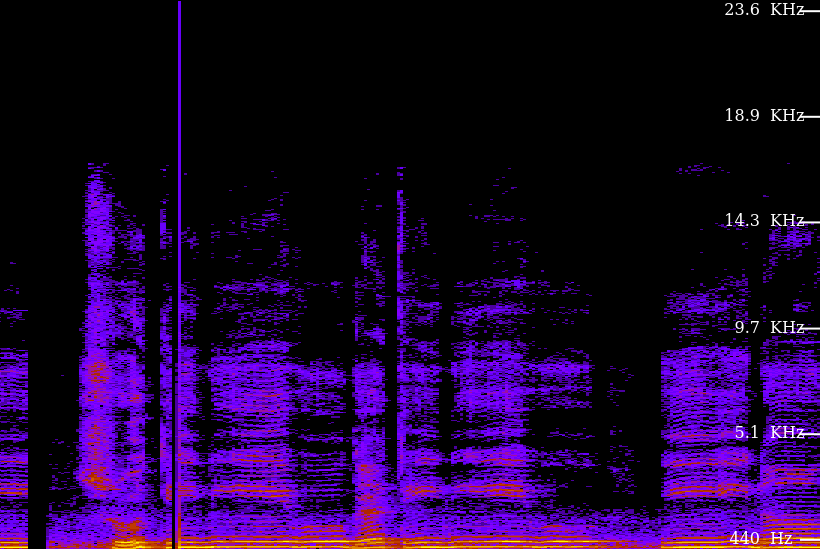
\includegraphics[width=1\columnwidth]{figs/original.46.png }
    \caption{Input audio to be filtered}
\end{figure}

The above figure depicts the spectogram of the audio with noise.


The frequencies which have very low intensities are represented as darker areas,and the frequencies that have high intensities in the sound are represented as orange, yellow areas.

\begin{figure}[H]
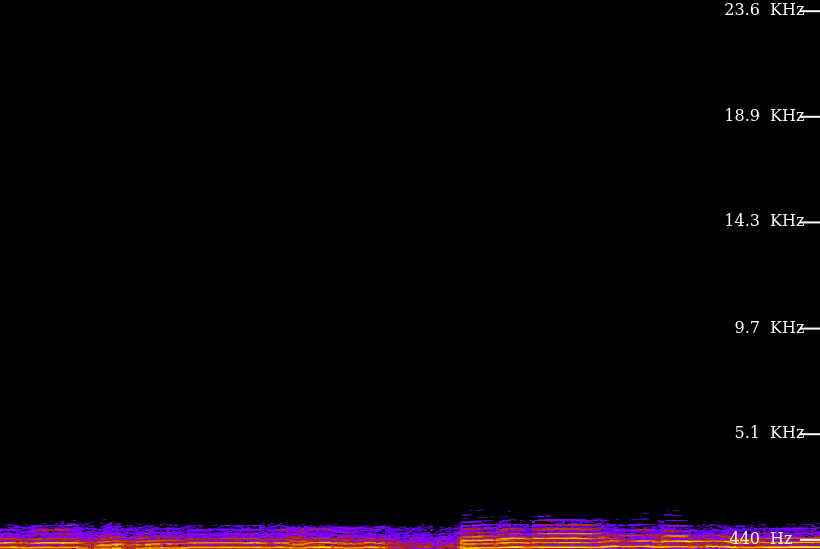
\includegraphics[width=1\columnwidth]{figs/filtered.46.png}
    \caption{Filtered audio}
\end{figure}
\end{enumerate}
he above figure depicts the spectogram of the filtered audio.


\section{Difference Equation}
\begin{enumerate}
\item Let
\begin{equation}
x(n) = \cbrak{\underset{\uparrow}{1},2,3,4,2,1} \label{2.1.46}
\end{equation}
Sketch $x(n)$. 
\item Let
\begin{multline}
y(n) + \frac{1}{2}y(n-1) = x(n) + x(n-2), 
\\
y(n) = 0, n < 0 \label{2.2.46}
\end{multline}
Sketch $y(n)$.\\
Solve\\
\solution  The values of $y\brak{n}$ are generated using C code from
\begin{lstlisting}
https://github.com/hemanth23ee/ASSIGNMENTS/blob/main/Audio%20filter%20assignment/codes/2_2.c
\end{lstlisting} 
The following python codes are used to plot \eqref{2.1.46} and \eqref{2.2.46}
\begin{lstlisting}
https://github.com/hemanth23ee/ASSIGNMENTS/blob/main/Audio%20filter%20assignment/codes/2_2.py   \\
https://github.com/hemanth23ee/ASSIGNMENTS/blob/main/Audio%20filter%20assignment/codes/2_2.1.py
\end{lstlisting}

\begin{figure}[H]
	\centering
	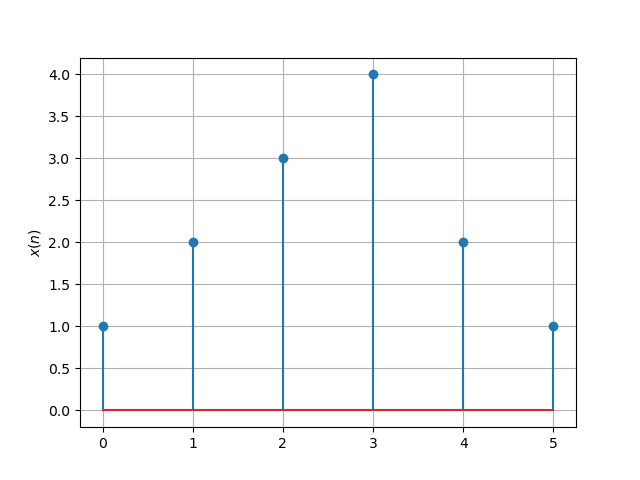
\includegraphics[width=\columnwidth]{figs/Plot_xn.png}
	\caption{Plot of $x(n)$ and $y(n)$}
	\label{xnyn.46}
\end{figure}
\begin{figure}[H]
	\centering
	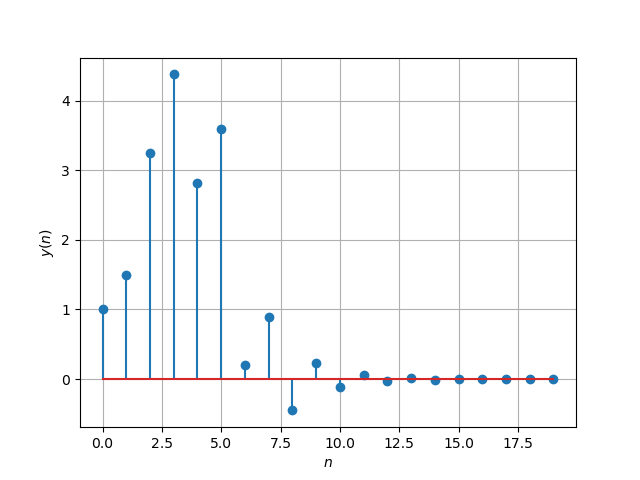
\includegraphics[width=\columnwidth]{figs/Plot_yn.png}
	\caption{Plot of $x(n)$ and $y(n)$}
	\label{xnyn.46}
\end{figure}
\end{enumerate}

\section{Z-Transform}

\begin{enumerate}[label=\thesection.\arabic*]
\item The $Z$-transform of $x(n)$ is defined as
%
\begin{equation}
\label{z_trans.46}
X(z)={\mathcal {Z}}\{x(n)\}=\sum _{n=-\infty }^{\infty }x(n)z^{-n}
\end{equation}
%
Show that
\begin{equation}
\label{shift1.46}
{\mathcal {Z}}\{x(n-1)\} = z^{-1}X(z)
\end{equation}
and find
\begin{equation}
	{\mathcal {Z}}\{x(n-k)\} 
\end{equation}
\solution From \eqref{z_trans.46},
\begin{align}
{\mathcal {Z}}\{x(n-k)\} &=\sum _{n=-\infty }^{\infty }x(n-1)z^{-n}
\\
&=\sum _{n=-\infty }^{\infty }x(n)z^{-n-1} = z^{-1}\sum _{n=-\infty }^{\infty }x(n)z^{-n}
\end{align}
resulting in \eqref{shift1.46}. Similarly, it can be shown that
%
\begin{equation}
\label{z_trans_shift.46}
	{\mathcal {Z}}\{x(n-k)\} = z^{-k}X(z)
\end{equation}

\item Find
%
\begin{equation}
H(z) = \frac{Y(z)}{X(z)}
\end{equation}
from  \eqref{2.2.46} assuming that the $Z$-transform is a linear operation.
\\
\solution  Applying \eqref{z_trans_shift.46} in \eqref{2.2.46},
\begin{align}
Y(z) + \frac{1}{2}z^{-1}Y(z) &= X(z)+z^{-2}X(z)
\\
\implies \frac{Y(z)}{X(z)} &= \frac{1 + z^{-2}}{1 + \frac{1}{2}z^{-1}}
\label{freq_resp.46}
\end{align}
%
\item Find the Z transform of 
\begin{equation}
\delta(n)
=
\begin{cases}
1 & n = 0
\\
0 & \text{otherwise}
\end{cases}
\end{equation}
and show that the $Z$-transform of
\begin{equation}
\label{unit_step.46}
u(n)
=
\begin{cases}
1 & n \ge 0
\\
0 & \text{otherwise}
\end{cases}
\end{equation}
is
\begin{equation}
U(z) = \frac{1}{1-z^{-1}}, \quad \abs{z} > 1
\end{equation}
\solution It is easy to show that
\begin{equation}
\delta(n) \system{Z} 1
\end{equation}
and from \eqref{unit_step.46},
\begin{align}
U(z) &= \sum _{n= 0}^{\infty}z^{-n}
\\
&=\frac{1}{1-z^{-1}}, \quad \abs{z} > 1
\end{align}
using the formula for the sum of an infinite geometric progression.
%
\item Show that 
\begin{equation}
\label{anun.46}
a^nu(n) \system{Z} \frac{1}{1-az^{-1}} \quad \abs{z} > \abs{a}
\end{equation}
\solution 
\begin{align}
	a^nu(n) &\system{Z} \sum_{n = 0}^{\infty}\brak{az^{-1}}^n \\
			&= \frac{1}{1-az^{-1}} \quad \abs{z} > \abs{a}
\end{align}
%
\item 
Let
\begin{equation}
H\brak{e^{\j \omega}} = H\brak{z = e^{\j \omega}}.
\end{equation}
Plot $\abs{H\brak{e^{\j \omega}}}$.  Comment.  $H(e^{\j \omega})$ is
known as the {\em Discret Time Fourier Transform} (DTFT) of $x(n)$.
\\
\solution The following python code is used to plot the magnitude of transfer function.
\begin{lstlisting}
https://github.com/hemanth23ee/ASSIGNMENTS/blob/main/Audio%20filter%20assignment/codes/3.5.py
\end{lstlisting}
Substituting $z = e^{j \omega}$ in \eqref{freq_resp.46}, we get
\begin{align}
	\left|H\brak{e^{j\omega}}\right| &= \left|\frac{1 + e^{-2j\omega}}{1 + \frac{1}{2}e^{-j\omega}}\right| \\
									  &= \sqrt{\frac{\brak{1 + \cos{2\omega}}^2 + \brak{\sin{2\omega}}^2}{\brak{1 + \frac{1}{2}\cos{\omega}}^2 + \brak{\frac{1}{2}\sin{\omega}}^2}}\\
									  &= \frac{4|\cos{\omega}|}{\sqrt{5 + 4\cos{\omega}}}
\end{align}
\begin{align}
	\left|H\brak{e^{j\brak{\omega + 2\pi}}}\right| &= \frac{4|\cos\brak{\omega + 2\pi}|}{\sqrt{5 + 4\cos\brak{\omega + 2\pi}}} \\
											   &= \frac{4|\cos{\omega}|}{\sqrt{5 + 4\cos{\omega}}} \\
											   &= \left|H\brak{e^{j\omega}}\right|	
\end{align}
Therefore its fundamental period is $2\pi$ , which verifies that DTFT of a signal is always periodic.

\begin{figure}[H]
\centering
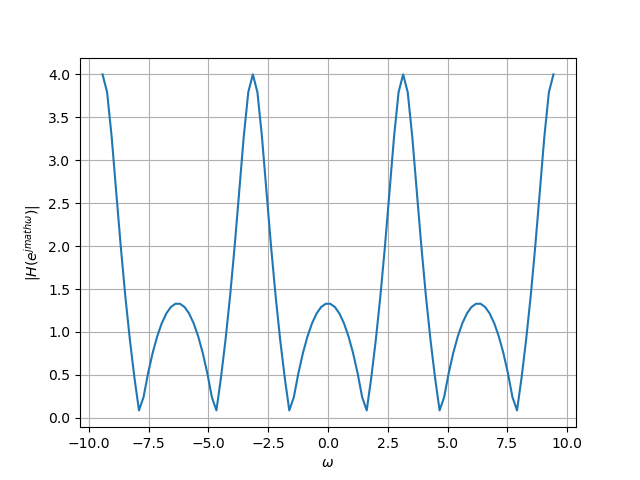
\includegraphics[width=\columnwidth]{figs/H(z)_3.5.png}
\caption{$\abs{H\brak{e^{j\omega}}}$}
\label{H(z)_3.5.46}
\end{figure}
\end{enumerate}

\section{Impulse Response}
\begin{enumerate}
\item \label{impulse_resp.46}
Find an expression for $h(n)$ using $H(z)$, given that 
%in Problem \ref{ztransab.46} and \eqref{anun.46}, given that
\begin{equation}
\label{impulse_resp.46}
h(n) \system{Z} H(z)
\end{equation}
and there is a one to one relationship between $h(n)$ and $H(z)$. $h(n)$ is known as the {\em impulse response} of the
system defined by \eqref{2.2.46}.
\\
\solution From \eqref{freq_resp.46},
\begin{align}
H(z) &= \frac{1}{1 + \frac{1}{2}z^{-1}} + \frac{ z^{-2}}{1 + \frac{1}{2}z^{-1}}
\\
\implies h(n) &= \brak{-\frac{1}{2}}^{n}u(n) + \brak{-\frac{1}{2}}^{n-2}u(n-2)
\end{align}
using \eqref{anun.46} and \eqref{z_trans_shift.46}.
\item Sketch $h(n)$. Is it bounded? Convergent? 
\\
\solution The python code used to plot $h\brak{n}$ can be obtained from 
\begin{lstlisting}
https://github.com/hemanth23ee/ASSIGNMENTS/blob/main/Audio%20filter%20assignment/codes/4.2.py
\end{lstlisting}
\begin{figure}[H]
\centering
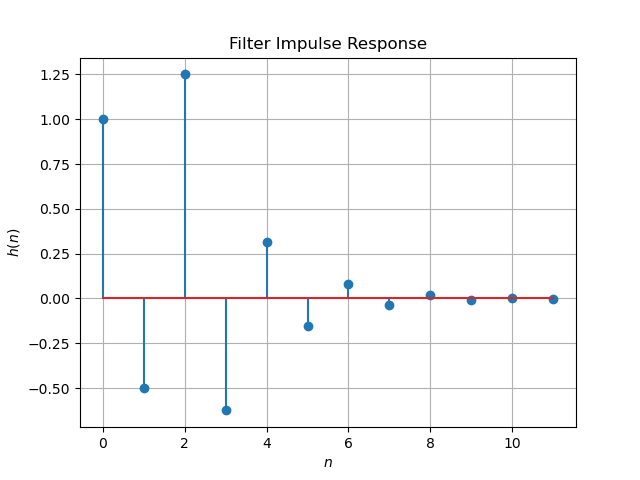
\includegraphics[width=\columnwidth]{figs/hn}
\caption{$h(n)$ as the inverse of $H(z)$}
\label{hn.46}
\end{figure}
%
\item The system with $h(n)$ is defined to be stable if
\begin{equation}
\sum_{n=-\infty}^{\infty}h(n) < \infty \label{stabilty_condn.46}
\end{equation}
Is the system defined by \eqref{2.2.46} stable for the impulse response in \eqref{impulse_resp.46}?\\
\solution For stable system \eqref{stabilty_condn.46} should converge.\\
By using ratio test
\begin{align}
    \lim_{n \to \infty}\left|\frac{h(n + 1)}{h(n)}\right|&<1 \\
\end{align}
For large $n$ 
\begin{align}
    u\brak{n}=u\brak{n-2}=1
\end{align}
\begin{align}
  \lim_{n \to \infty}  \brak{\frac{h(n + 1)}{h(n)}} = 1/2 <1
\end{align}
Therefore it converges. Hence it is stable.
\item 
Compute and sketch $h(n)$ using 
\begin{equation}
\label{iir_filter_h.46}
h(n) + \frac{1}{2}h(n-1) = \delta(n) + \delta(n-2), 
\end{equation}
%
This is the definition of $h(n)$.
\\
\solution\\
Definition of $h\brak{n}$: The output of the system when $\delta\brak{n}$ is given as input.\\

The following code plots Fig. \ref{hndef.46}. Note that this is the same as Fig. 
\ref{hn.46}. 

\begin{lstlisting}
https://github.com/hemanth23ee/ASSIGNMENTS/blob/main/Audio%20filter%20assignment/codes/4.2.py
\end{lstlisting}
\begin{figure}[!ht]
\centering
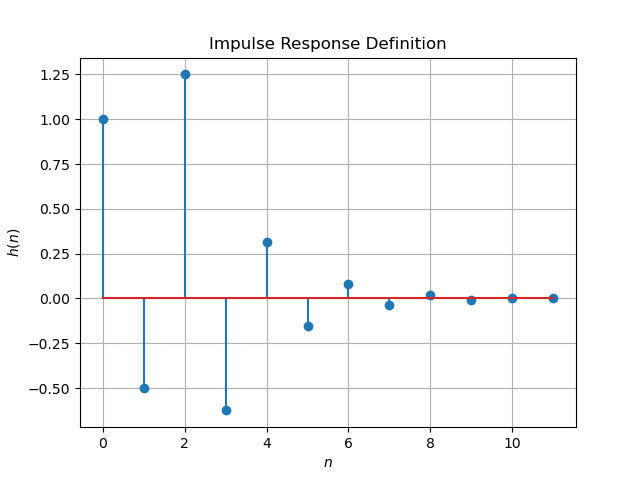
\includegraphics[width=\columnwidth]{figs/hndef}
\caption{$h(n)$ from the definition is same as \figref{fig:hn}}
\label{hndef.46}
\end{figure}
%
\item Compute 
%
\begin{equation}
\label{convolution.46}
y(n) = x(n)*h(n) = \sum_{n=-\infty}^{\infty}x(k)h(n-k)
\end{equation}
%
Comment. The operation in \eqref{convolution.46} is known as
{\em convolution}.
%
\\
\solution The python code used to plot Fig. \ref{ynconv.46} can be obtained from link below. Note that this is the same as 
$y(n)$ in  Fig. 
\ref{xnyn.46}. 
%
\begin{lstlisting}
https://github.com/hemanth23ee/ASSIGNMENTS/blob/main/Audio%20filter%20assignment/codes/4.5.py
\end{lstlisting}
\begin{figure}[H]
\centering
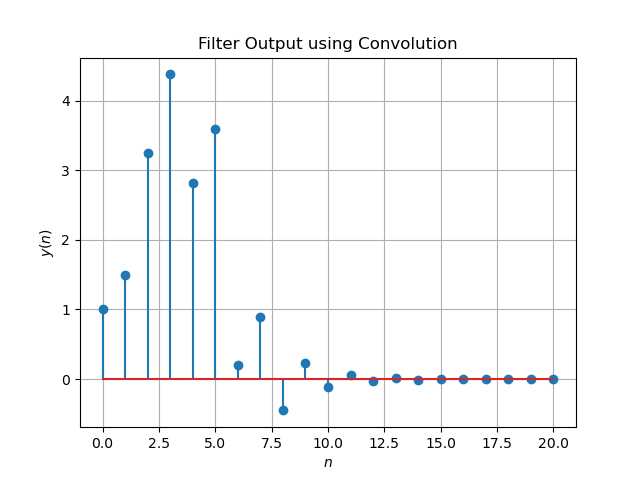
\includegraphics[width=\columnwidth]{figs/y_by_conv.png}
\caption{$y(n)$ from the definition of convolution}
\label{ynconv.46}
\end{figure}

\item Show that
\begin{equation}
y(n) =  \sum_{n=-\infty}^{\infty}x(n-k)h(k)
\end{equation}
\solution
In \eqref{convolution.46}, we substitute $k = n - k$ to get
\begin{align}
y\brak{n} &= \sum_{k=-\infty}^{\infty}x\brak{k}h\brak{n - k} \\
		  &= \sum_{n - k=-\infty}^{\infty}x\brak{n - k}h\brak{k} \\
		  &= \sum_{k=-\infty}^{\infty}x\brak{n - k}h\brak{k}
\end{align}
\end{enumerate}


\newpage
\section{DFT and FFT}
\begin{enumerate}
\item
Compute
\begin{equation}
X(k) \define \sum _{n=0}^{N-1}x(n) e^{-\j2\pi kn/N}, \quad k = 0,1,\dots, N-1
\end{equation}
and $H(k)$ using $h(n)$.
\item Compute 
\begin{equation}
Y(k) = X(k)H(k)
\label{fp.46}
\end{equation}
\item Compute
\begin{equation}
y\brak{n}={\frac {1}{N}}\sum _{k=0}^{N-1}Y\brak{k}\cdot e^{\j 2\pi kn/N},\quad n = 0,1,\dots, N-1
\label{inv-ft.46}
\end{equation}

\solution The above three questions are solved using the code from
\begin{lstlisting}
https://github.com/hemanth23ee/ASSIGNMENTS/blob/main/Audio%20filter%20assignment/codes/5_sol.py
\end{lstlisting}

\item Repeat the previous exercise by computing $X(k), H(k)$ and $y(n)$ through FFT and IFFT.
\solution The solution of this question can be found in the code from
\begin{lstlisting}
https://github.com/hemanth23ee/ASSIGNMENTS/blob/main/Audio%20filter%20assignment/codes/5.4.py  
\end{lstlisting}
This code verifies the result by plotting the obtained result with the result obtained by IDFT.
\begin{figure}[H]
\centering
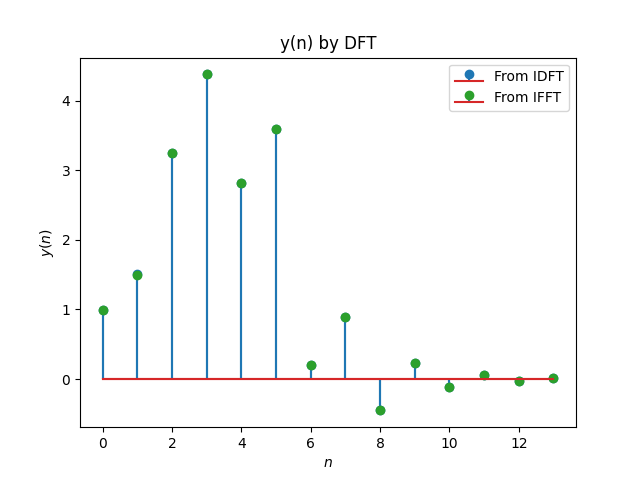
\includegraphics[width=\columnwidth]{figs/yn_verf_5.4.png}
\caption{$y(n)$ obtained from IDFT and IFFT is plotted and verified}
\label{yn_verf_5.4.46}
\end{figure}

\item Wherever possible, express all the above equations as matrix equations.\\
\solution The DFT matrix is defined as : 
\begin{align}
	\mtx{W} = 
	\begin{pmatrix}
		\omega^0 & \omega^0 & \ldots & \omega^0 \\
		\omega^0 & \omega^1 & \ldots & \omega^{N - 1} \\
		\vdots & \vdots & \ddots & \vdots \\
		\omega^0 & \omega^{N - 1} & \ldots & \omega^{(N -1)(N - 1)}
	\end{pmatrix}
\end{align}
where $\omega=e^{-\frac{j2\pi}{N}}$ . Now any DFT equation can be written as
\begin{align}
    \mtx{X} = \mtx{W}\mtx{x}
\end{align}
\noindent where
\begin{align}
	\mtx{x} = 
	\begin{pmatrix}
		x(0) \\ x(1) \\ \vdots \\ x(n - 1)
	\end{pmatrix}
\end{align}
\begin{align}
	\mtx{X} = 
	\begin{pmatrix}
		X(0) \\ X(1) \\ \vdots \\ X(n - 1)
	\end{pmatrix}
\end{align}
Thus we can rewrite  \eqref{fp.46} as:
\begin{align}
	\mtx{Y} = \mtx{X}\odot\mtx{H} = \brak{\mtx{W}\mtx{x}}\odot\brak{\mtx{W}\mtx{h}}
\end{align}
where the $\odot$ represents the Hadamard product which performs element-wise multiplication.
\end{enumerate}

The below code computes $y\brak{n}$ by DFT Matrix and then plots it.
\begin{lstlisting}
https://github.com/hemanth23ee/ASSIGNMENTS/blob/main/Audio%20filter%20assignment/codes/5.5.py
\end{lstlisting}
\begin{figure}[H]
\centering
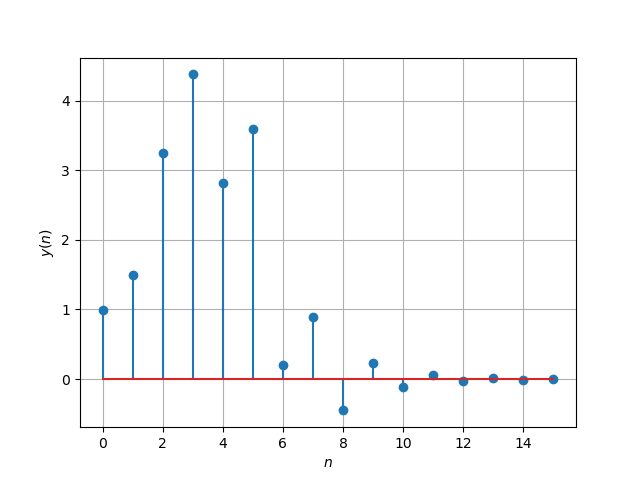
\includegraphics[width=\columnwidth]{figs/yn_DFT_matrix.png}
\caption{$y(n)$ obtained from DFT Matrix}
\label{yn_DFT_matrix.46}
\end{figure}

\section{\underline{EXERCISES}}
\noindent Answer the following questions by looking at the python code in Problem \ref{audio_filter.46}.


\begin{enumerate}
\item
The command
\begin{lstlisting}
	output_signal = signal.lfilter(b, a, input_signal)
	\end{lstlisting}
in Problem \ref{audio_filter.46} is executed through the following difference equation
\begin{equation}
\label{iir_filter_gen.46}
 \sum _{m=0}^{M}a\brak{m}y\brak{n-m}=\sum _{k=0}^{N}b\brak{k}x\brak{n-k} 
\end{equation}
%
where the input signal is $x(n)$ and the output signal is $y(n)$ with initial values all 0. Replace
\textbf{signal. filtfilt} with your own routine and verify.\\

\solution The below code gives the output of an Audio Filter without using the built in function signal.lfilter.
\begin{lstlisting}
https://github.com/hemanth23ee/ASSIGNMENTS/blob/main/Audio%20filter%20assignment/codes/6.1.py 
\end{lstlisting}
\begin{figure}[H]
\centering
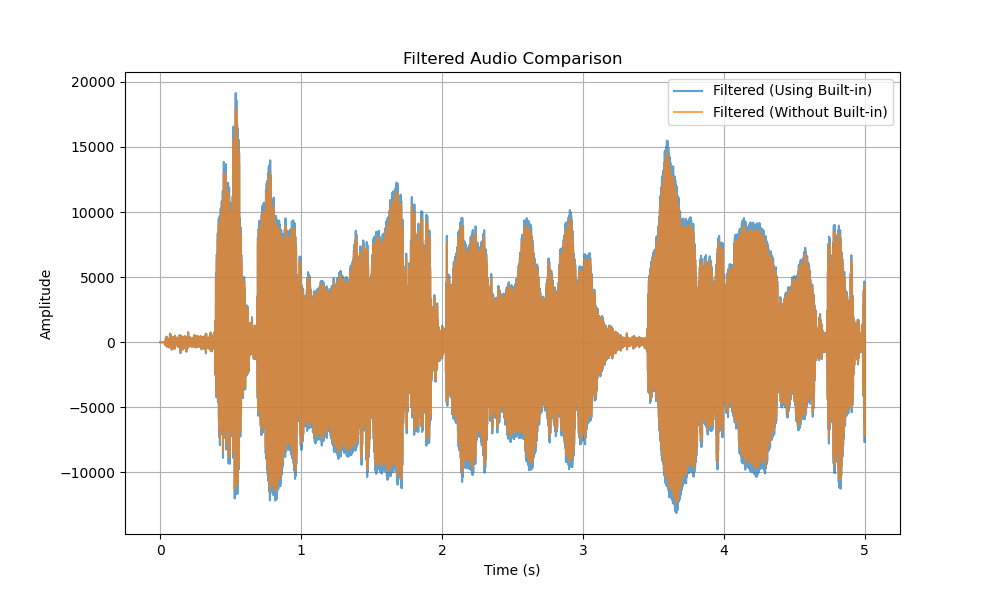
\includegraphics[width=1.2\columnwidth]{figs/Audio_Filter_verf.png}
\caption{Both the outputs using and without using function overlap}
\label{6.1.46}
\end{figure}





\item Repeat all the exercises in the previous sections for the above $a$ and $b$.\\
\solution The code in \ref{audio_filter.46} generates the values of $a$ and $b$  which can be used to generate a difference equation.\\
And,
\begin{align}
    M &= 5\\
    N&=5
\end{align}
From \ref{iir_filter_gen.46} 
\begin{align}
    &a\brak{0}y\brak{n} + a\brak{1}y\brak{n-1}+a\brak{2}y\brak{n-2}+a\brak{3}\\ \notag &y\brak{n-3} + a\brak{4}y\brak{n-4} =   b\brak{0}x\brak{n} + b\brak{1}x\brak{n-1}\\ \notag &+b\brak{2}x\brak{n-2}+b\brak{3}x\brak{n-3} + b\brak{4}x\brak{n-4} 
\end{align}
Difference Equation is given by :
\begin{align}
	&y(n) - \brak{3.63}y(n - 1) + \brak{4.95}y(n - 2) \nonumber \\
	&- \brak{3.012}y(n - 3) + \brak{0.689}y(n - 4) \nonumber \\
	&= \brak{2.15\times 10^{-5}}x(n) + \brak{8.61 \times 10^{-5}}x(n - 1) \nonumber \\
	&+ \brak{1.291 \times 10^{-5}}x(n - 2) + \brak{8.608 \times 10^{-5}}x(n - 3) \nonumber \\
	&+ \brak{2.152 \times 10^{-5}}x(n - 4)
\end{align}
From \eqref{iir_filter_gen.46} 
\begin{align}
    H(z) &= \frac{b_0 + b_1 z^{-1} + b_2 z^{-2} + \ldots + b_M z^{-N}}{a_0 + a_1 z^{-1} + a_2 z^{-2} + \ldots + a_N z^{-M}}\\
    H(z) &= \frac{\sum_{k = 0}^{N}b(k)z^{-k}}{\sum_{k = 0}^{M}a(k)z^{-k}} \label{trans-func.46}
\end{align}
Partial fraction on \eqref{trans-func.46} can be generalised as:
\begin{align}
    H\brak{z}&= \sum_{i}\frac{r(i)}{1 - p(i)z^{-1}} + \sum_{j}k(j)z^{-j}
	\label{trans-func-pfe.46}
\end{align}
Now,
\begin{align}
    a^{n}u\brak{n} \system{Z} \frac{1}{1-az^{-1}} \label{res-1.46}\\
    \delta\brak{n-k} \system{Z} z^{-k}\label{res-2.46}
\end{align}
Taking inverse z transform of \eqref{trans-func-pfe.46} by using \eqref{res-1.46} and \eqref{res-2.46}
\begin{align}
h(n) &= \sum_{i}r(i)[p(i)]^nu(n) + \sum_{j}k(j)\delta(n - j)
	\label{h-n-expr.46}
\end{align}
The below code computes the values of $r\brak{i},p\brak{i} , k\brak{i}$ and plots $h\brak{n}$
\begin{lstlisting}
https://github.com/hemanth23ee/ASSIGNMENTS/blob/main/Audio%20filter%20assignment/codes/6.2.py
\end{lstlisting}
\begin{table}[H]
    \centering
    \renewcommand\thetable{1}
    \setlength{\extrarowheight}{9pt}
    \resizebox{0.51\textwidth}{!}{
    \begin{tabular}{|c|c|c|}
    \hline
    \textbf{$r\brak{i}$} & \textbf{$p\brak{i}$} & \textbf{$k\brak{i}$} \\ \hline
    $0.06558697-0.15997359j$ &0.87507075+0.0480371j&$3.124\times10^{-5}$  \\ \hline
    $0.06558697-0.15997359j$ &0.87507075+0.0480371j&$-$  \\ \hline
    $-0.06559183+0.02744514j$ &0.93885135+0.12442455j&$-$  \\ \hline
    $-0.06559183+0.02744514j$ &0.93885135+0.12442455j&$-$  \\ \hline
    \end{tabular}}
    \caption{Values of $ r(i) , p(i) , k(i)$}
    \label{tab:values of r(i) , p(i) , k(i)}
    \end{table}


\textbf{Stability of h(n)}:\\
According to \eqref{stabilty_condn.46}
\begin{align}
H\brak{z} &= \sum_{n = 0}^{\infty} h\brak{n}z^{-n}\\
H(1)&= \sum_{n = 0}^{\infty}h(n)  = \frac{\sum_{k = 0}^{N}b(k)}{\sum_{k = 0}^{M}a(k)}< \infty
\end{align}
As both $a\brak{k}$ and $b\brak{k}$ are finite length sequences they converge.\\
The below code plots Filter frequency response
\begin{lstlisting}
https://github.com/hemanth23ee/ASSIGNMENTS/blob/main/Audio%20filter%20assignment/codes/6_filter_response.py
\end{lstlisting}
\begin{figure}[H]
\centering
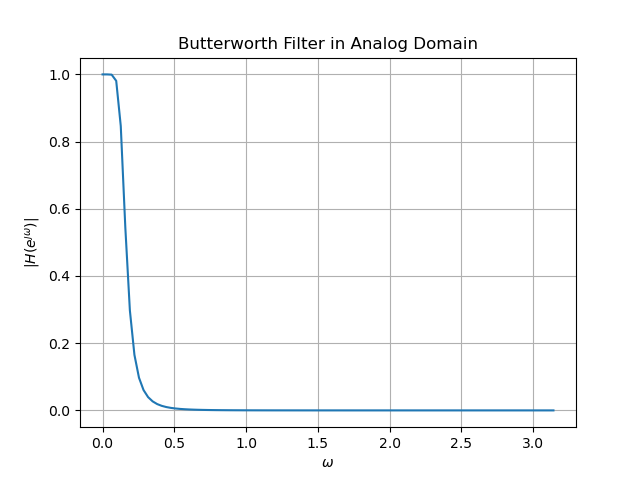
\includegraphics[width=1\columnwidth]{figs/Filter_Response.png}
\caption{Frequency Response of Audio Filter}
\label{H(w)_6.46}
\end{figure}
The below code plots the Butterworth Filter in analog domain by using bilinear transform.
\begin{align}
    z=\frac{1+sT/2}{1-sT/2}
\end{align}
\begin{lstlisting}
https://github.com/hemanth23ee/ASSIGNMENTS/blob/main/Audio%20filter%20assignment/codes/analog_filt.py
\end{lstlisting}
\begin{figure}[H]
\centering
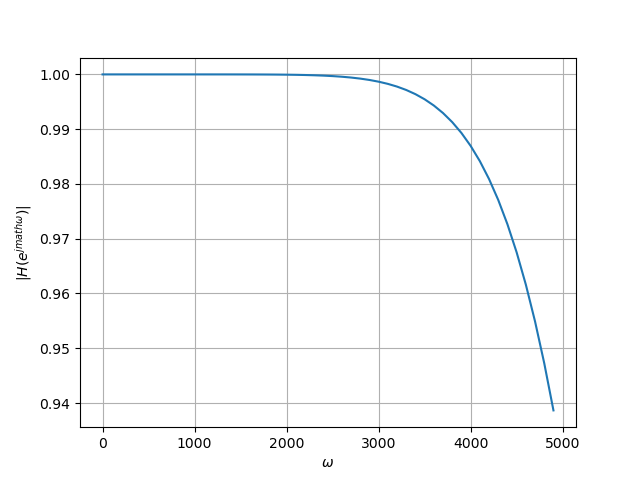
\includegraphics[width=1\columnwidth]{figs/Butterworth_analog.png}
\caption{Butterworth Filter Frequency response in analog domain}
\label{H(w)_6.46.1}
\end{figure}



The below code plots the Pole-Zero Plot of the frequency response.
\begin{lstlisting}
https://github.com/hemanth23ee/ASSIGNMENTS/blob/main/Audio%20filter%20assignment/codes/6.2_pole-zero.py
\end{lstlisting}
\begin{figure}[H]
\centering
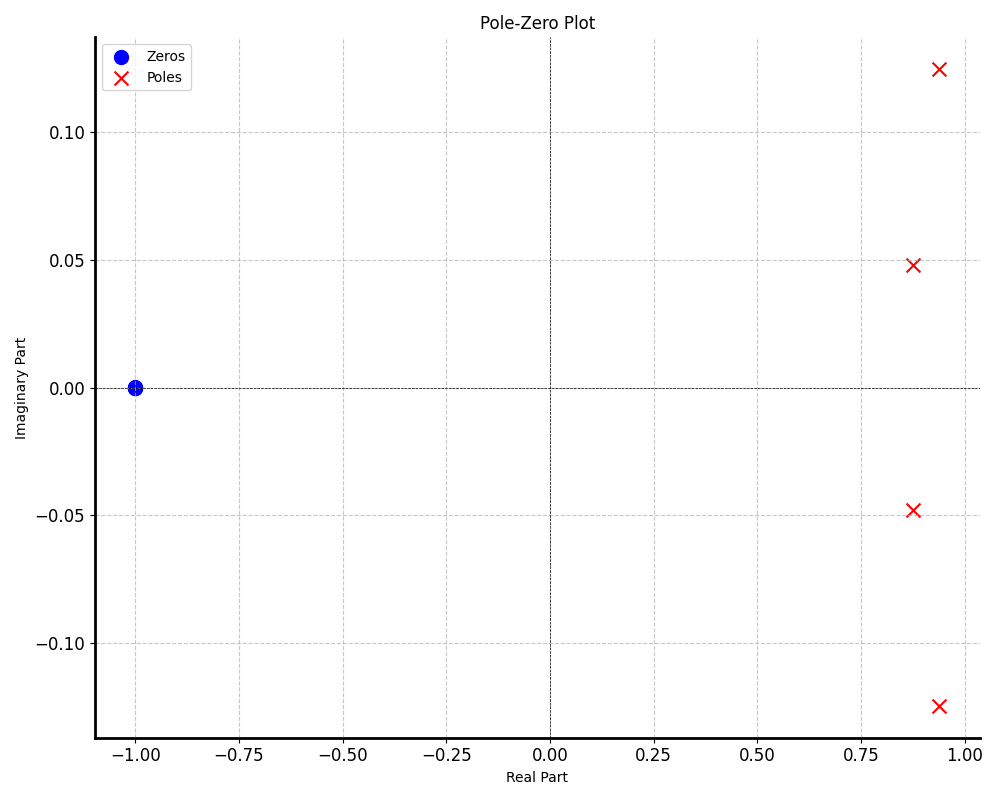
\includegraphics[width=1\columnwidth]{figs/Pole_Zero_Plt.png}
\caption{There are complex poles. So $h\brak{n}$ should be damped sinusoid.}
\label{pole_zero_6.2.46}
\end{figure}

\begin{figure}[H]
\centering
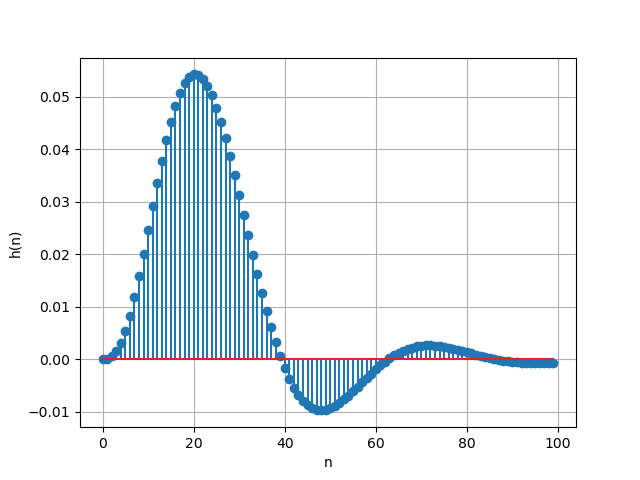
\includegraphics[width=\columnwidth]{figs/h(n)_6.2.png}
\caption{h(n) of Audio Filter.It is a damped sinusoid.}
\label{6.2_hn.46}
\end{figure}


\item What is the sampling frequency of the input signal?\\
\solution The Sampling Frequency is 44.1KHz
\item
What is type, order and  cutoff-frequency of the above butterworth filter
\\
\solution The given butterworth filter is lowpass with order=4 and cutoff-frequency=1kHz.

\item
Modify the code with different input parameters and get the best possible output.

\solution
A better filtering was found on setting the order of the filter to be 5.

\end{enumerate}


\end{document}
